% Created by tikzDevice version 0.10.1 on 2017-12-04 16:18:40
% !TEX encoding = UTF-8 Unicode
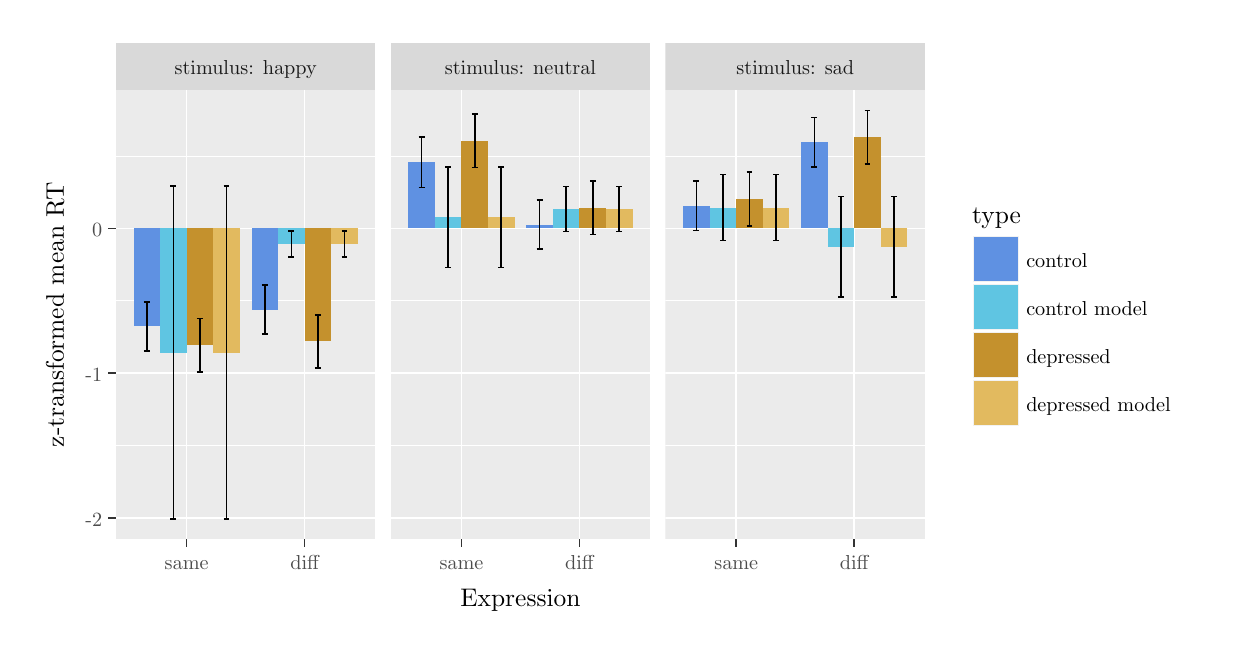
\begin{tikzpicture}[x=1pt,y=1pt]
\definecolor{fillColor}{RGB}{255,255,255}
\path[use as bounding box,fill=fillColor,fill opacity=0.00] (0,0) rectangle (433.62,216.81);
\begin{scope}
\path[clip] (  0.00,  0.00) rectangle (433.62,216.81);
\definecolor{drawColor}{RGB}{255,255,255}
\definecolor{fillColor}{RGB}{255,255,255}

\path[draw=drawColor,line width= 0.6pt,line join=round,line cap=round,fill=fillColor] (  0.00,  0.00) rectangle (433.62,216.81);
\end{scope}
\begin{scope}
\path[clip] ( 31.87, 31.92) rectangle (125.67,194.25);
\definecolor{fillColor}{gray}{0.92}

\path[fill=fillColor] ( 31.87, 31.92) rectangle (125.67,194.25);
\definecolor{drawColor}{RGB}{255,255,255}

\path[draw=drawColor,line width= 0.3pt,line join=round] ( 31.87, 65.78) --
	(125.67, 65.78);

\path[draw=drawColor,line width= 0.3pt,line join=round] ( 31.87,118.12) --
	(125.67,118.12);

\path[draw=drawColor,line width= 0.3pt,line join=round] ( 31.87,170.45) --
	(125.67,170.45);

\path[draw=drawColor,line width= 0.6pt,line join=round] ( 31.87, 39.62) --
	(125.67, 39.62);

\path[draw=drawColor,line width= 0.6pt,line join=round] ( 31.87, 91.95) --
	(125.67, 91.95);

\path[draw=drawColor,line width= 0.6pt,line join=round] ( 31.87,144.28) --
	(125.67,144.28);

\path[draw=drawColor,line width= 0.6pt,line join=round] ( 57.45, 31.92) --
	( 57.45,194.25);

\path[draw=drawColor,line width= 0.6pt,line join=round] (100.08, 31.92) --
	(100.08,194.25);
\definecolor{fillColor}{RGB}{226,186,95}

\path[fill=fillColor] ( 67.04, 99.42) rectangle ( 76.64,144.28);
\definecolor{fillColor}{RGB}{196,145,45}

\path[fill=fillColor] ( 57.45,102.04) rectangle ( 67.04,144.28);
\definecolor{fillColor}{RGB}{95,197,226}

\path[fill=fillColor] ( 47.86, 99.42) rectangle ( 57.45,144.28);
\definecolor{fillColor}{RGB}{95,145,226}

\path[fill=fillColor] ( 38.27,108.87) rectangle ( 47.86,144.28);
\definecolor{fillColor}{RGB}{226,186,95}

\path[fill=fillColor] (109.68,138.68) rectangle (119.27,144.28);
\definecolor{fillColor}{RGB}{196,145,45}

\path[fill=fillColor] (100.08,103.41) rectangle (109.68,144.28);
\definecolor{fillColor}{RGB}{95,197,226}

\path[fill=fillColor] ( 90.49,138.68) rectangle (100.08,144.28);
\definecolor{fillColor}{RGB}{95,145,226}

\path[fill=fillColor] ( 80.90,114.95) rectangle ( 90.49,144.28);
\definecolor{drawColor}{RGB}{0,0,0}

\path[draw=drawColor,line width= 0.6pt,line join=round] ( 70.77,159.55) --
	( 72.91,159.55);

\path[draw=drawColor,line width= 0.6pt,line join=round] ( 71.84,159.55) --
	( 71.84, 39.30);

\path[draw=drawColor,line width= 0.6pt,line join=round] ( 70.77, 39.30) --
	( 72.91, 39.30);

\path[draw=drawColor,line width= 0.6pt,line join=round] ( 61.18,111.72) --
	( 63.31,111.72);

\path[draw=drawColor,line width= 0.6pt,line join=round] ( 62.25,111.72) --
	( 62.25, 92.36);

\path[draw=drawColor,line width= 0.6pt,line join=round] ( 61.18, 92.36) --
	( 63.31, 92.36);

\path[draw=drawColor,line width= 0.6pt,line join=round] ( 51.59,159.55) --
	( 53.72,159.55);

\path[draw=drawColor,line width= 0.6pt,line join=round] ( 52.66,159.55) --
	( 52.66, 39.30);

\path[draw=drawColor,line width= 0.6pt,line join=round] ( 51.59, 39.30) --
	( 53.72, 39.30);

\path[draw=drawColor,line width= 0.6pt,line join=round] ( 42.00,117.77) --
	( 44.13,117.77);

\path[draw=drawColor,line width= 0.6pt,line join=round] ( 43.06,117.77) --
	( 43.06, 99.98);

\path[draw=drawColor,line width= 0.6pt,line join=round] ( 42.00, 99.98) --
	( 44.13, 99.98);

\path[draw=drawColor,line width= 0.6pt,line join=round] (113.41,143.42) --
	(115.54,143.42);

\path[draw=drawColor,line width= 0.6pt,line join=round] (114.47,143.42) --
	(114.47,133.93);

\path[draw=drawColor,line width= 0.6pt,line join=round] (113.41,133.93) --
	(115.54,133.93);

\path[draw=drawColor,line width= 0.6pt,line join=round] (103.82,113.09) --
	(105.95,113.09);

\path[draw=drawColor,line width= 0.6pt,line join=round] (104.88,113.09) --
	(104.88, 93.73);

\path[draw=drawColor,line width= 0.6pt,line join=round] (103.82, 93.73) --
	(105.95, 93.73);

\path[draw=drawColor,line width= 0.6pt,line join=round] ( 94.22,143.42) --
	( 96.35,143.42);

\path[draw=drawColor,line width= 0.6pt,line join=round] ( 95.29,143.42) --
	( 95.29,133.93);

\path[draw=drawColor,line width= 0.6pt,line join=round] ( 94.22,133.93) --
	( 96.35,133.93);

\path[draw=drawColor,line width= 0.6pt,line join=round] ( 84.63,123.87) --
	( 86.76,123.87);

\path[draw=drawColor,line width= 0.6pt,line join=round] ( 85.70,123.87) --
	( 85.70,106.03);

\path[draw=drawColor,line width= 0.6pt,line join=round] ( 84.63,106.03) --
	( 86.76,106.03);
\end{scope}
\begin{scope}
\path[clip] (131.17, 31.92) rectangle (224.96,194.25);
\definecolor{fillColor}{gray}{0.92}

\path[fill=fillColor] (131.17, 31.92) rectangle (224.96,194.25);
\definecolor{drawColor}{RGB}{255,255,255}

\path[draw=drawColor,line width= 0.3pt,line join=round] (131.17, 65.78) --
	(224.96, 65.78);

\path[draw=drawColor,line width= 0.3pt,line join=round] (131.17,118.12) --
	(224.96,118.12);

\path[draw=drawColor,line width= 0.3pt,line join=round] (131.17,170.45) --
	(224.96,170.45);

\path[draw=drawColor,line width= 0.6pt,line join=round] (131.17, 39.62) --
	(224.96, 39.62);

\path[draw=drawColor,line width= 0.6pt,line join=round] (131.17, 91.95) --
	(224.96, 91.95);

\path[draw=drawColor,line width= 0.6pt,line join=round] (131.17,144.28) --
	(224.96,144.28);

\path[draw=drawColor,line width= 0.6pt,line join=round] (156.75, 31.92) --
	(156.75,194.25);

\path[draw=drawColor,line width= 0.6pt,line join=round] (199.38, 31.92) --
	(199.38,194.25);
\definecolor{fillColor}{RGB}{226,186,95}

\path[fill=fillColor] (166.34,144.28) rectangle (175.93,148.35);
\definecolor{fillColor}{RGB}{196,145,45}

\path[fill=fillColor] (156.75,144.28) rectangle (166.34,176.01);
\definecolor{fillColor}{RGB}{95,197,226}

\path[fill=fillColor] (147.15,144.28) rectangle (156.75,148.35);
\definecolor{fillColor}{RGB}{95,145,226}

\path[fill=fillColor] (137.56,144.28) rectangle (147.15,168.15);
\definecolor{fillColor}{RGB}{226,186,95}

\path[fill=fillColor] (208.97,144.28) rectangle (218.56,151.29);
\definecolor{fillColor}{RGB}{196,145,45}

\path[fill=fillColor] (199.38,144.28) rectangle (208.97,151.81);
\definecolor{fillColor}{RGB}{95,197,226}

\path[fill=fillColor] (189.79,144.28) rectangle (199.38,151.29);
\definecolor{fillColor}{RGB}{95,145,226}

\path[fill=fillColor] (180.19,144.28) rectangle (189.79,145.65);
\definecolor{drawColor}{RGB}{0,0,0}

\path[draw=drawColor,line width= 0.6pt,line join=round] (170.07,166.58) --
	(172.20,166.58);

\path[draw=drawColor,line width= 0.6pt,line join=round] (171.13,166.58) --
	(171.13,130.11);

\path[draw=drawColor,line width= 0.6pt,line join=round] (170.07,130.11) --
	(172.20,130.11);

\path[draw=drawColor,line width= 0.6pt,line join=round] (160.48,185.69) --
	(162.61,185.69);

\path[draw=drawColor,line width= 0.6pt,line join=round] (161.54,185.69) --
	(161.54,166.33);

\path[draw=drawColor,line width= 0.6pt,line join=round] (160.48,166.33) --
	(162.61,166.33);

\path[draw=drawColor,line width= 0.6pt,line join=round] (150.88,166.58) --
	(153.01,166.58);

\path[draw=drawColor,line width= 0.6pt,line join=round] (151.95,166.58) --
	(151.95,130.11);

\path[draw=drawColor,line width= 0.6pt,line join=round] (150.88,130.11) --
	(153.01,130.11);

\path[draw=drawColor,line width= 0.6pt,line join=round] (141.29,177.27) --
	(143.42,177.27);

\path[draw=drawColor,line width= 0.6pt,line join=round] (142.36,177.27) --
	(142.36,159.03);

\path[draw=drawColor,line width= 0.6pt,line join=round] (141.29,159.03) --
	(143.42,159.03);

\path[draw=drawColor,line width= 0.6pt,line join=round] (212.70,159.41) --
	(214.83,159.41);

\path[draw=drawColor,line width= 0.6pt,line join=round] (213.77,159.41) --
	(213.77,143.16);

\path[draw=drawColor,line width= 0.6pt,line join=round] (212.70,143.16) --
	(214.83,143.16);

\path[draw=drawColor,line width= 0.6pt,line join=round] (203.11,161.51) --
	(205.24,161.51);

\path[draw=drawColor,line width= 0.6pt,line join=round] (204.18,161.51) --
	(204.18,142.11);

\path[draw=drawColor,line width= 0.6pt,line join=round] (203.11,142.11) --
	(205.24,142.11);

\path[draw=drawColor,line width= 0.6pt,line join=round] (193.52,159.41) --
	(195.65,159.41);

\path[draw=drawColor,line width= 0.6pt,line join=round] (194.58,159.41) --
	(194.58,143.16);

\path[draw=drawColor,line width= 0.6pt,line join=round] (193.52,143.16) --
	(195.65,143.16);

\path[draw=drawColor,line width= 0.6pt,line join=round] (183.92,154.54) --
	(186.06,154.54);

\path[draw=drawColor,line width= 0.6pt,line join=round] (184.99,154.54) --
	(184.99,136.75);

\path[draw=drawColor,line width= 0.6pt,line join=round] (183.92,136.75) --
	(186.06,136.75);
\end{scope}
\begin{scope}
\path[clip] (230.46, 31.92) rectangle (324.25,194.25);
\definecolor{fillColor}{gray}{0.92}

\path[fill=fillColor] (230.46, 31.92) rectangle (324.25,194.25);
\definecolor{drawColor}{RGB}{255,255,255}

\path[draw=drawColor,line width= 0.3pt,line join=round] (230.46, 65.78) --
	(324.25, 65.78);

\path[draw=drawColor,line width= 0.3pt,line join=round] (230.46,118.12) --
	(324.25,118.12);

\path[draw=drawColor,line width= 0.3pt,line join=round] (230.46,170.45) --
	(324.25,170.45);

\path[draw=drawColor,line width= 0.6pt,line join=round] (230.46, 39.62) --
	(324.25, 39.62);

\path[draw=drawColor,line width= 0.6pt,line join=round] (230.46, 91.95) --
	(324.25, 91.95);

\path[draw=drawColor,line width= 0.6pt,line join=round] (230.46,144.28) --
	(324.25,144.28);

\path[draw=drawColor,line width= 0.6pt,line join=round] (256.04, 31.92) --
	(256.04,194.25);

\path[draw=drawColor,line width= 0.6pt,line join=round] (298.67, 31.92) --
	(298.67,194.25);
\definecolor{fillColor}{RGB}{226,186,95}

\path[fill=fillColor] (265.63,144.28) rectangle (275.22,151.81);
\definecolor{fillColor}{RGB}{196,145,45}

\path[fill=fillColor] (256.04,144.28) rectangle (265.63,154.87);
\definecolor{fillColor}{RGB}{95,197,226}

\path[fill=fillColor] (246.45,144.28) rectangle (256.04,151.81);
\definecolor{fillColor}{RGB}{95,145,226}

\path[fill=fillColor] (236.85,144.28) rectangle (246.45,152.43);
\definecolor{fillColor}{RGB}{226,186,95}

\path[fill=fillColor] (308.27,137.68) rectangle (317.86,144.28);
\definecolor{fillColor}{RGB}{196,145,45}

\path[fill=fillColor] (298.67,144.28) rectangle (308.27,177.17);
\definecolor{fillColor}{RGB}{95,197,226}

\path[fill=fillColor] (289.08,137.68) rectangle (298.67,144.28);
\definecolor{fillColor}{RGB}{95,145,226}

\path[fill=fillColor] (279.49,144.28) rectangle (289.08,175.39);
\definecolor{drawColor}{RGB}{0,0,0}

\path[draw=drawColor,line width= 0.6pt,line join=round] (269.36,163.77) --
	(271.49,163.77);

\path[draw=drawColor,line width= 0.6pt,line join=round] (270.43,163.77) --
	(270.43,139.86);

\path[draw=drawColor,line width= 0.6pt,line join=round] (269.36,139.86) --
	(271.49,139.86);

\path[draw=drawColor,line width= 0.6pt,line join=round] (259.77,164.55) --
	(261.90,164.55);

\path[draw=drawColor,line width= 0.6pt,line join=round] (260.84,164.55) --
	(260.84,145.19);

\path[draw=drawColor,line width= 0.6pt,line join=round] (259.77,145.19) --
	(261.90,145.19);

\path[draw=drawColor,line width= 0.6pt,line join=round] (250.18,163.77) --
	(252.31,163.77);

\path[draw=drawColor,line width= 0.6pt,line join=round] (251.24,163.77) --
	(251.24,139.86);

\path[draw=drawColor,line width= 0.6pt,line join=round] (250.18,139.86) --
	(252.31,139.86);

\path[draw=drawColor,line width= 0.6pt,line join=round] (240.58,161.33) --
	(242.72,161.33);

\path[draw=drawColor,line width= 0.6pt,line join=round] (241.65,161.33) --
	(241.65,143.54);

\path[draw=drawColor,line width= 0.6pt,line join=round] (240.58,143.54) --
	(242.72,143.54);

\path[draw=drawColor,line width= 0.6pt,line join=round] (312.00,155.85) --
	(314.13,155.85);

\path[draw=drawColor,line width= 0.6pt,line join=round] (313.06,155.85) --
	(313.06,119.51);

\path[draw=drawColor,line width= 0.6pt,line join=round] (312.00,119.51) --
	(314.13,119.51);

\path[draw=drawColor,line width= 0.6pt,line join=round] (302.40,186.87) --
	(304.53,186.87);

\path[draw=drawColor,line width= 0.6pt,line join=round] (303.47,186.87) --
	(303.47,167.47);

\path[draw=drawColor,line width= 0.6pt,line join=round] (302.40,167.47) --
	(304.53,167.47);

\path[draw=drawColor,line width= 0.6pt,line join=round] (292.81,155.85) --
	(294.94,155.85);

\path[draw=drawColor,line width= 0.6pt,line join=round] (293.88,155.85) --
	(293.88,119.51);

\path[draw=drawColor,line width= 0.6pt,line join=round] (292.81,119.51) --
	(294.94,119.51);

\path[draw=drawColor,line width= 0.6pt,line join=round] (283.22,184.29) --
	(285.35,184.29);

\path[draw=drawColor,line width= 0.6pt,line join=round] (284.28,184.29) --
	(284.28,166.50);

\path[draw=drawColor,line width= 0.6pt,line join=round] (283.22,166.50) --
	(285.35,166.50);
\end{scope}
\begin{scope}
\path[clip] ( 31.87,194.25) rectangle (125.67,211.31);
\definecolor{fillColor}{gray}{0.85}

\path[fill=fillColor] ( 31.87,194.25) rectangle (125.67,211.31);
\definecolor{drawColor}{gray}{0.10}

\node[text=drawColor,anchor=base,inner sep=0pt, outer sep=0pt, scale=  0.73] at ( 78.77,199.75) {stimulus: happy};
\end{scope}
\begin{scope}
\path[clip] (131.17,194.25) rectangle (224.96,211.31);
\definecolor{fillColor}{gray}{0.85}

\path[fill=fillColor] (131.17,194.25) rectangle (224.96,211.31);
\definecolor{drawColor}{gray}{0.10}

\node[text=drawColor,anchor=base,inner sep=0pt, outer sep=0pt, scale=  0.73] at (178.06,199.75) {stimulus: neutral};
\end{scope}
\begin{scope}
\path[clip] (230.46,194.25) rectangle (324.25,211.31);
\definecolor{fillColor}{gray}{0.85}

\path[fill=fillColor] (230.46,194.25) rectangle (324.25,211.31);
\definecolor{drawColor}{gray}{0.10}

\node[text=drawColor,anchor=base,inner sep=0pt, outer sep=0pt, scale=  0.73] at (277.36,199.75) {stimulus: sad};
\end{scope}
\begin{scope}
\path[clip] (  0.00,  0.00) rectangle (433.62,216.81);
\definecolor{drawColor}{gray}{0.20}

\path[draw=drawColor,line width= 0.6pt,line join=round] ( 57.45, 29.17) --
	( 57.45, 31.92);

\path[draw=drawColor,line width= 0.6pt,line join=round] (100.08, 29.17) --
	(100.08, 31.92);
\end{scope}
\begin{scope}
\path[clip] (  0.00,  0.00) rectangle (433.62,216.81);
\definecolor{drawColor}{gray}{0.30}

\node[text=drawColor,anchor=base,inner sep=0pt, outer sep=0pt, scale=  0.73] at ( 57.45, 20.91) {same};

\node[text=drawColor,anchor=base,inner sep=0pt, outer sep=0pt, scale=  0.73] at (100.08, 20.91) {diff};
\end{scope}
\begin{scope}
\path[clip] (  0.00,  0.00) rectangle (433.62,216.81);
\definecolor{drawColor}{gray}{0.20}

\path[draw=drawColor,line width= 0.6pt,line join=round] (156.75, 29.17) --
	(156.75, 31.92);

\path[draw=drawColor,line width= 0.6pt,line join=round] (199.38, 29.17) --
	(199.38, 31.92);
\end{scope}
\begin{scope}
\path[clip] (  0.00,  0.00) rectangle (433.62,216.81);
\definecolor{drawColor}{gray}{0.30}

\node[text=drawColor,anchor=base,inner sep=0pt, outer sep=0pt, scale=  0.73] at (156.75, 20.91) {same};

\node[text=drawColor,anchor=base,inner sep=0pt, outer sep=0pt, scale=  0.73] at (199.38, 20.91) {diff};
\end{scope}
\begin{scope}
\path[clip] (  0.00,  0.00) rectangle (433.62,216.81);
\definecolor{drawColor}{gray}{0.20}

\path[draw=drawColor,line width= 0.6pt,line join=round] (256.04, 29.17) --
	(256.04, 31.92);

\path[draw=drawColor,line width= 0.6pt,line join=round] (298.67, 29.17) --
	(298.67, 31.92);
\end{scope}
\begin{scope}
\path[clip] (  0.00,  0.00) rectangle (433.62,216.81);
\definecolor{drawColor}{gray}{0.30}

\node[text=drawColor,anchor=base,inner sep=0pt, outer sep=0pt, scale=  0.73] at (256.04, 20.91) {same};

\node[text=drawColor,anchor=base,inner sep=0pt, outer sep=0pt, scale=  0.73] at (298.67, 20.91) {diff};
\end{scope}
\begin{scope}
\path[clip] (  0.00,  0.00) rectangle (433.62,216.81);
\definecolor{drawColor}{gray}{0.30}

\node[text=drawColor,anchor=base east,inner sep=0pt, outer sep=0pt, scale=  0.73] at ( 26.92, 36.59) {-2};

\node[text=drawColor,anchor=base east,inner sep=0pt, outer sep=0pt, scale=  0.73] at ( 26.92, 88.92) {-1};

\node[text=drawColor,anchor=base east,inner sep=0pt, outer sep=0pt, scale=  0.73] at ( 26.92,141.25) {0};
\end{scope}
\begin{scope}
\path[clip] (  0.00,  0.00) rectangle (433.62,216.81);
\definecolor{drawColor}{gray}{0.20}

\path[draw=drawColor,line width= 0.6pt,line join=round] ( 29.12, 39.62) --
	( 31.87, 39.62);

\path[draw=drawColor,line width= 0.6pt,line join=round] ( 29.12, 91.95) --
	( 31.87, 91.95);

\path[draw=drawColor,line width= 0.6pt,line join=round] ( 29.12,144.28) --
	( 31.87,144.28);
\end{scope}
\begin{scope}
\path[clip] (  0.00,  0.00) rectangle (433.62,216.81);
\definecolor{drawColor}{RGB}{0,0,0}

\node[text=drawColor,anchor=base,inner sep=0pt, outer sep=0pt, scale=  0.92] at (178.06,  7.83) {Expression};
\end{scope}
\begin{scope}
\path[clip] (  0.00,  0.00) rectangle (433.62,216.81);
\definecolor{drawColor}{RGB}{0,0,0}

\node[text=drawColor,rotate= 90.00,anchor=base,inner sep=0pt, outer sep=0pt, scale=  0.92] at ( 13.08,113.08) {z-transformed mean RT};
\end{scope}
\begin{scope}
\path[clip] (  0.00,  0.00) rectangle (433.62,216.81);
\definecolor{fillColor}{RGB}{255,255,255}

\path[fill=fillColor] (335.63, 66.75) rectangle (428.12,159.42);
\end{scope}
\begin{scope}
\path[clip] (  0.00,  0.00) rectangle (433.62,216.81);
\definecolor{drawColor}{RGB}{0,0,0}

\node[text=drawColor,anchor=base west,inner sep=0pt, outer sep=0pt, scale=  0.92] at (341.32,146.15) {type};
\end{scope}
\begin{scope}
\path[clip] (  0.00,  0.00) rectangle (433.62,216.81);
\definecolor{drawColor}{RGB}{255,255,255}
\definecolor{fillColor}{gray}{0.95}

\path[draw=drawColor,line width= 0.6pt,line join=round,line cap=round,fill=fillColor] (341.32,124.47) rectangle (358.67,141.82);
\end{scope}
\begin{scope}
\path[clip] (  0.00,  0.00) rectangle (433.62,216.81);
\definecolor{fillColor}{RGB}{95,145,226}

\path[fill=fillColor] (342.04,125.18) rectangle (357.96,141.11);
\end{scope}
\begin{scope}
\path[clip] (  0.00,  0.00) rectangle (433.62,216.81);
\definecolor{drawColor}{RGB}{255,255,255}
\definecolor{fillColor}{gray}{0.95}

\path[draw=drawColor,line width= 0.6pt,line join=round,line cap=round,fill=fillColor] (341.32,107.13) rectangle (358.67,124.47);
\end{scope}
\begin{scope}
\path[clip] (  0.00,  0.00) rectangle (433.62,216.81);
\definecolor{fillColor}{RGB}{95,197,226}

\path[fill=fillColor] (342.04,107.84) rectangle (357.96,123.76);
\end{scope}
\begin{scope}
\path[clip] (  0.00,  0.00) rectangle (433.62,216.81);
\definecolor{drawColor}{RGB}{255,255,255}
\definecolor{fillColor}{gray}{0.95}

\path[draw=drawColor,line width= 0.6pt,line join=round,line cap=round,fill=fillColor] (341.32, 89.78) rectangle (358.67,107.13);
\end{scope}
\begin{scope}
\path[clip] (  0.00,  0.00) rectangle (433.62,216.81);
\definecolor{fillColor}{RGB}{196,145,45}

\path[fill=fillColor] (342.04, 90.49) rectangle (357.96,106.42);
\end{scope}
\begin{scope}
\path[clip] (  0.00,  0.00) rectangle (433.62,216.81);
\definecolor{drawColor}{RGB}{255,255,255}
\definecolor{fillColor}{gray}{0.95}

\path[draw=drawColor,line width= 0.6pt,line join=round,line cap=round,fill=fillColor] (341.32, 72.44) rectangle (358.67, 89.78);
\end{scope}
\begin{scope}
\path[clip] (  0.00,  0.00) rectangle (433.62,216.81);
\definecolor{fillColor}{RGB}{226,186,95}

\path[fill=fillColor] (342.04, 73.15) rectangle (357.96, 89.07);
\end{scope}
\begin{scope}
\path[clip] (  0.00,  0.00) rectangle (433.62,216.81);
\definecolor{drawColor}{RGB}{0,0,0}

\node[text=drawColor,anchor=base west,inner sep=0pt, outer sep=0pt, scale=  0.73] at (360.84,130.12) {control};
\end{scope}
\begin{scope}
\path[clip] (  0.00,  0.00) rectangle (433.62,216.81);
\definecolor{drawColor}{RGB}{0,0,0}

\node[text=drawColor,anchor=base west,inner sep=0pt, outer sep=0pt, scale=  0.73] at (360.84,112.77) {control model};
\end{scope}
\begin{scope}
\path[clip] (  0.00,  0.00) rectangle (433.62,216.81);
\definecolor{drawColor}{RGB}{0,0,0}

\node[text=drawColor,anchor=base west,inner sep=0pt, outer sep=0pt, scale=  0.73] at (360.84, 95.43) {depressed};
\end{scope}
\begin{scope}
\path[clip] (  0.00,  0.00) rectangle (433.62,216.81);
\definecolor{drawColor}{RGB}{0,0,0}

\node[text=drawColor,anchor=base west,inner sep=0pt, outer sep=0pt, scale=  0.73] at (360.84, 78.08) {depressed model};
\end{scope}
\end{tikzpicture}
